\documentclass[a4paper,12pt]{article}
\usepackage[utf8]{inputenc}
\usepackage[T2A]{fontenc}
\usepackage[russian,english]{babel}
\usepackage{graphicx}
\usepackage{amsmath, amssymb, amsthm}
\usepackage{algorithm}
\usepackage{algpseudocode}
\usepackage{geometry}
\usepackage{enumitem}
\usepackage{hyperref}
\usepackage{mathtools}
\usepackage{subcaption}
\usepackage{wrapfig}
\usepackage{float}
\usepackage{tikz}
\usetikzlibrary{arrows.meta, shapes, positioning, shadows, fit, decorations.markings}
\geometry{left=20mm, right=20mm, top=20mm, bottom=20mm}

\newtheorem{theorem}{Теорема}
\newtheorem{lemma}{Лемма}
\newtheorem{definition}{Определение}
\newtheorem{proposition}{Утверждение}

\title{Локальные свойства нейронных сетей через призму гессианов слоёв}
\author{Максим Большим}
\date{\today}

\begin{document}

\maketitle

\begin{abstract}
  В данной работе представлен новый подход к анализу нейронных сетей, основанный на исследовании локальных
  свойств их параметрического пространства с помощью матриц Гессе. Введено понятие локального гессиана,
  позволяющее изучать геометрию функционального пространства отдельных слоев нейронной сети. Предложены
  методы количественной оценки таких феноменов, как переобучение и недостаточная аппроксимирующая способность
  моделей, через спектральные характеристики локальных гессианов. Проведённый анализ 147 экспериментов на 37
  датасетах показал существенные закономерности в структуре локальных матриц гессиана на различных этапах обучения.
  Разработанный математический аппарат позволяет глубже понимать внутренние процессы в глубоких нейронных
  сетях во время их обучения. а так же представляет из себя отличную основу для поиска слабых мест в архитектуре
\end{abstract}

\section{Введение}

Глубокие нейронные сети продемонстрировали выдающиеся результаты во многих областях, включая компьютерное
зрение, обработку естественного языка и прочие задачи машинного обучения \cite{lecun2015deep,
goodfellow2016deep}. Однако, несмотря на их практический успех, остаётся открытым вопрос о том, почему одни
архитектуры превосходят другие и как систематически улучшать дизайн нейронных сетей. Эмпирический подход,
основанный на методе проб и ошибок, становится всё более затратным с ростом размеров моделей и объёмов данных.

Ряд работ показывает, что анализ кривизны ландшафта функции потерь через гессианы и родственные спектральные
инструменты может пролить свет на динамику обучения и обобщающую способность моделей
\cite{sagun2017empirical, maheswaranathan2019universality, lee2019wide, arora2019finegrained}. В настоящем
исследовании выдвигается тезис о том, что локальные свойства параметрического пространства нейронной сети
могут предоставить ценную информацию о внутренних процессах в модели без необходимости полной переобучения
\cite{poole2016transient}. Конкретно, мы предлагаем использовать локальные матрицы Гессе — матрицы вторых
производных целевой функции по параметрам отдельных слоёв — для анализа геометрии пространства параметров.

Концепция локального гессиана позволяет формализовать и количественно измерить геометрические свойства
пространства параметров в окрестности точки оптимизации. В частности, мы показываем, что спектральные
свойства локального гессиана, такие как распределение собственных значений и их структура
\cite{ghorbani2019investigation}, тесно связаны с функциональными свойствами соответствующих слоёв нейронной сети.

Основные вклады настоящей работы:
\begin{itemize}
  \item Введение математически строгого определения локального гессиана для функциональных блоков нейронной сети
  \item Детальный анализ спектральных свойств локальных гессианов в процессе обучения нейронных сетей
  \item Исследование геометрической интерпретации пространства параметров через призму локальных гессианов
\end{itemize}

Полученные результаты не только углубляют наше теоретическое понимание глубоких нейронных сетей, но и
открывают новые перспективы для изучения их внутренней динамики.

\section{Математический аппарат нейронных сетей}

\subsection{Определение и структура нейронной сети}

\begin{definition}
  Нейронная сеть $\mathcal{F}: \mathbb{R}^d \rightarrow \mathbb{R}^m$ представляет собой параметризованную
  функцию с параметрами $\theta \in \mathbb{R}^P$, отображающую входные данные $x \in \mathbb{R}^d$ в
  выходное пространство через последовательность функциональных преобразований. Обозначим через
  $\mathcal{F}(x; \theta)$ результат применения сети к входным данным при заданных параметрах $\theta$.
\end{definition}

\begin{definition}
  Функциональным блоком (слоем) $C_i$ нейронной сети $\mathcal{F}$ называется пара модулей $(P_i, A_i)$, где:
  \begin{itemize}
    \item $P_i: \mathbb{R}^{d_i} \times \mathbb{R}^{p_i} \rightarrow \mathbb{R}^{q_i}$ -- параметризованное
      преобразование с параметрами $\theta_i \in \mathbb{R}^{p_i}$.
    \item $A_i: \mathbb{R}^{q_i} \rightarrow \mathbb{R}^{q_i}$ -- функция активации (потенциально тождественная)
  \end{itemize}
\end{definition}

\begin{definition}
  Нейронную сеть $\mathcal{F}$ можно представить как композицию $n$ функциональных блоков:
  \begin{equation}
    \mathcal{F}(x; \theta) = (C_n \circ C_{n-1} \circ \ldots \circ C_1)(x),
  \end{equation}
  где $C_i(z) = A_i(P_i(z; \theta_i))$ для входа $z$ и $\theta = \{\theta_1, \theta_2, \ldots, \theta_n\}$ --
  полный набор параметров сети.
\end{definition}

Такое представление нейронной сети позволяет нам анализировать каждый функциональный блок отдельно, что важно
для локального анализа свойств сети. Декомпозиция сложной модели на более простые составляющие является
ключевым методологическим приемом, который позволяет применить инструменты спектрального анализа к отдельным
компонентам.

\subsection{Промежуточные представления и функции активации}

\begin{definition}
  Промежуточным представлением $z_i$ называется вход в блок $C_i$:
  \begin{equation}
    z_i =
    \begin{cases}
      x, & \text{если } i = 1 \\
      (C_{i-1} \circ \ldots \circ C_1)(x), & \text{если } i > 1
    \end{cases}
  \end{equation}

  Соответственно, выход блока $C_i$ обозначается как:
  \begin{equation}
    y_i = C_i(z_i) = A_i(P_i(z_i; \theta_i))
  \end{equation}
\end{definition}

Промежуточные представления играют важную роль в анализе нейронных сетей, поскольку они содержат информацию о
том, как входной сигнал преобразуется на каждом этапе обработки. Особый интерес представляет изучение
геометрии этих промежуточных представлений и их взаимосвязь с параметрами соответствующих слоев.

\begin{definition}
  Для блока $C_i$ определим локальную скалярную функцию $S_i: \mathbb{R}^{p_i} \rightarrow \mathbb{R}$ как:
  \begin{equation}
    S_i(\theta_i) = \varphi(A_i(P_i(z_i; \theta_i))),
  \end{equation}
  где $\varphi: \mathbb{R}^{q_i} \rightarrow \mathbb{R}$ -- функция агрегации, обычно $\varphi(y) =
  \sum_{j=1}^{q_i} y_j$.
\end{definition}

Локальная скалярная функция представляет собой способ оценки влияния параметров конкретного слоя на его выход
при фиксированном входе. Эта функция будет ключевой для определения локального гессиана в следующем разделе.

\subsection{Типичные реализации в нейросетях}

В контексте современных нейронных сетей часто используются следующие реализации компонентов:
\begin{itemize}
  \item $P_i$ -- линейное преобразование $P_i(z_i; \theta_i) = W_i z_i + b_i$, где $\theta_i = \{W_i, b_i\}$
  \item $A_i$ -- нелинейная функция активации, например, ReLU, Sigmoid или Tanh
  \item $\varphi(y_i) = \sum_{j=1}^{q_i} y_{i,j}$ -- суммирование всех компонент выходного вектора
\end{itemize}

Эти определения и обозначения будут использоваться во всех последующих разделах данной работы для обеспечения
математической строгости и последовательности.

\section{Локальные гессианы нейронной сети}

\subsection{Определение локального гессиана}

\begin{definition}
  Локальной матрицей Гессе $H_i \in \mathbb{R}^{p_i \times p_i}$ для блока $C_i$ называется матрица вторых
  производных скалярной функции $S_i$ по параметрам $\theta_i$:
  \begin{equation}
    H_i = \nabla_{\theta_i}^2 S_i(\theta_i) = \left[ \frac{\partial^2 S_i(\theta_i)}{\partial \theta_{i,j}
    \partial \theta_{i,k}} \right]_{j,k=1}^{p_i}
  \end{equation}
\end{definition}

Локальный гессиан представляет собой локальную кривизну функции отклика слоя относительно изменения его
параметров. Анализ этой матрицы позволяет получить информацию о:

\begin{itemize}
  \item Степени нелинейности преобразования, выполняемого слоем
  \item Взаимосвязи между параметрами и их влиянии на выход слоя
  \item Геометрических свойствах пространства параметров
  \item Чувствительности слоя к малым изменениям параметров
\end{itemize}

Конструкция локального гессиана имеет глубокое геометрическое значение. В дифференциальной геометрии гессиан
функции в точке определяет квадратичную форму, которая аппроксимирует локальную кривизну поверхности уровня
этой функции. В контексте нейронных сетей локальный гессиан характеризует кривизну функционального отклика
слоя в пространстве его параметров \cite{dangel2019modular}.

\subsection{Эффективное вычисление локальных гессианов}

Анализ нейронных сетей с использованием матриц Гессе представляет собой эффективный инструмент, однако из-за
квадратичной зависимости размера данной матрицы от числа параметров её прямое применение часто оказывается
вычислительно непрактичным. В связи с этим на практике широко применяются различные методы аппроксимации
гессиана \cite{carlon2024, hare2024, martens2010, nocedal1980}. В данном разделе предлагается методика работы
с гессианами, позволяющая обойти указанные ограничения.

Для эффективного вычисления локальных гессианов предлагается алгоритм, основанный на последовательном
вычислении строк матрицы.

\begin{lemma}
  Элементы матрицы Гессе $H_i$ можно вычислять последовательно по строкам:
  \begin{equation}
    \begin{aligned}
      g_i &= \nabla_{\theta_i} S_i(\theta_i) = \left[ \frac{\partial S_i}{\partial \theta_{i,j}} \right]_{j=1}^{p_i} \\
      H_i[j,:] &= \nabla_{\theta_i} g_{i,j} = \nabla_{\theta_i} \left( \frac{\partial S_i}{\partial
      \theta_{i,j}} \right)
    \end{aligned}
  \end{equation}
\end{lemma}

\begin{proof}
  По определению матрицы Гессе, её элемент $H_i[j,k]$ равен:
  \begin{equation}
    H_i[j,k] = \frac{\partial^2 S_i(\theta_i)}{\partial \theta_{i,j} \partial \theta_{i,k}}
  \end{equation}

  Если обозначить $g_{i,j} = \frac{\partial S_i}{\partial \theta_{i,j}}$, то
  \begin{equation}
    H_i[j,k] = \frac{\partial g_{i,j}}{\partial \theta_{i,k}}
  \end{equation}

  Таким образом, $j$-я строка $H_i$ представляет собой градиент $j$-й компоненты градиента функции $S_i$.
\end{proof}

Это позволяет значительно сократить вычислительные затраты при работе с большими моделями, так как не требует
одновременного хранения в памяти всей матрицы Гессе размером $p_i \times p_i$.

Предложенный метод особенно важен при анализе современных глубоких нейронных сетей, содержащих миллионы
параметров, поскольку полная матрица Гессе для таких моделей была бы непомерно большой. Локальный подход не
только делает вычисления практически реализуемыми, но и позволяет сосредоточиться на анализе отдельных
компонентов сети, что часто более информативно, чем глобальный анализ.

\subsection{Алгоритм вычисления локальных гессианов}

\begin{algorithm}
  \caption{Вычисление локальных матриц Гессе}
  \begin{algorithmic}[1]
    \Require Нейронная сеть $\mathcal{F}$, входные данные $x \in \mathbb{R}^d$, функция агрегации $\varphi$
    \Ensure Набор локальных матриц Гессе $\{H_1, H_2, \ldots, H_n\}$

    \State Разбить $\mathcal{F}$ на функциональные блоки $\{C_1, C_2, \ldots, C_n\}$, где $C_i = (P_i, A_i)$

    \For{$i = 1$ до $n$}
    \State Вычислить $z_i = (C_{i-1} \circ \ldots \circ C_1)(x)$ \Comment{Вход в блок $C_i$}
    \State Вычислить $y_i = A_i(P_i(z_i; \theta_i))$ \Comment{Выход блока $C_i$}
    \State Вычислить $S_i = \varphi(y_i)$ \Comment{Скалярная функция блока}

    \State Вычислить градиент $g_i = \nabla_{\theta_i} S_i$

    \State Инициализировать $H_i \in \mathbb{R}^{p_i \times p_i}$ нулевой матрицей

    \For{$j = 1$ до $p_i$}
    \If{$g_{i,j}$ зависит от $\theta_i$}
    \State Вычислить $H_i[j,:] = \nabla_{\theta_i} g_{i,j}$
    \EndIf
    \EndFor
    \EndFor

    \State \Return $\{H_1, H_2, \ldots, H_n\}$
  \end{algorithmic}
\end{algorithm}

\subsection{Математические детали реализации}

\subsubsection{Вычисление градиента $g_i$}
В контексте автоматического дифференцирования градиент $g_i$ вычисляется как:
\begin{equation}
  g_i = \nabla_{\theta_i} S_i = \frac{\partial S_i}{\partial y_i} \cdot \frac{\partial y_i}{\partial P_i}
  \cdot \frac{\partial P_i}{\partial \theta_i}
\end{equation}

где:
\begin{itemize}
  \item $\frac{\partial S_i}{\partial y_i} = \nabla_{y_i} \varphi(y_i)$ -- градиент функции агрегации
  \item $\frac{\partial y_i}{\partial P_i} = \nabla_{P_i} A_i(P_i)$ -- якобиан активационной функции
  \item $\frac{\partial P_i}{\partial \theta_i}$ -- якобиан параметризованного преобразования по его параметрам
\end{itemize}

\begin{figure}[ht]
  \centering
  \begin{tikzpicture}[
      box/.style={draw, minimum width=1.2cm, minimum height=3cm, thick},
      smallbox/.style={draw, minimum width=1cm, minimum height=3cm, thick},
      arrow/.style={-Stealth, line width=1pt},
    ]
    % 1) Стрелка над всеми слоями
    \draw[arrow] (-2,4) -- (10,4);
    \node[draw, fill=white, rounded corners, drop shadow] at (4,4.5)
    {Направления вычислений};

    % 2) Область вычислений гессиана
    \draw[rounded corners, thick] (3,-0.5) rectangle (7,3.5);

    % 3) Подпись под блоком
    \node[draw, fill=white, rounded corners, drop shadow] at (5,-0.8) {область вычисления гессиана};

    % 4) Слои
    \node[box]      (L0) at (-1,1.5) {$layer_0$};
    \node[smallbox] (L1) at (2,1.5) {$\ldots$};
    \node[smallbox] (L2) at (4,1.5) {$\ldots$};
    \node[smallbox] (L3) at (6,1.5) {$\ldots$};
    \node[box]      (Ln) at (9,1.5) {$layer_n$};

    % 5) Стрелки между слоями
    \draw[arrow] (-3,1.5) -- (L0);
    \draw[arrow] (L0) -- (L1);
    \draw[arrow] (L1) -- (L2);
    \draw[arrow] (L2) -- (L3);
    \draw[arrow] (L3) -- (Ln);
    \draw[arrow] (Ln) -- (10,1.5);
  \end{tikzpicture}
  \caption{Визуализация вычисления локального гессиана}
  \label{fig:layerwise_hessian}
\end{figure}

\subsubsection{Вычисление строк матрицы Гессе}
Для каждой компоненты $j$ градиента $g_i$ вычисляется её градиент по параметрам $\theta_i$:
\begin{equation}
  H_i[j,:] = \nabla_{\theta_i} g_{i,j} = \nabla_{\theta_i} \left( \frac{\partial S_i}{\partial \theta_{i,j}} \right)
\end{equation}

Это требует повторного применения автоматического дифференцирования к каждой компоненте градиента.

\subsection{Спектральный анализ гессиана для выявления структуры пространства параметров}

Спектральный анализ локальных гессианов предоставляет важный инструмент для понимания геометрии пространства
параметров. Распределение и структура собственных значений гессиана отражают ключевые свойства локальной
кривизны функции, что особенно важно для анализа степени обусловленности задачи оптимизации \cite{sagun2016,
liaomahoney2021}.

Для каждого локального гессиана $H_i$ можно вычислить:

\begin{equation}
  H_i = U_i\Lambda_i U_i^T = \sum_{j=1}^{p_i} \lambda_{i,j} u_{i,j} u_{i,j}^T
\end{equation}

где $\lambda_{i,j}$ - $j$-е собственное значение, а $u_{i,j}$ - соответствующий собственный вектор.

Характерные показатели спектра гессиана включают:

\begin{itemize}
  \item \textbf{Следы гессиана:} $\text{tr}(H_i) = \sum_{j=1}^{p_i} \lambda_{i,j}$ — сумма собственных
    значений, отражающая общую кривизну
  \item \textbf{Определитель гессиана:} $\det(H_i) = \prod_{j=1}^{p_i} \lambda_{i,j}$ — произведение
    собственных значений
  \item \textbf{Условное число:} $\kappa(H_i) = \frac{\lambda_{i,\max}}{\lambda_{i,\min}}$ — отношение
    максимального собственного значения к минимальному (для ненулевых значений)
  \item \textbf{Эффективный ранг:} $r_{\text{eff}}(H_i) = \frac{\sum_{j} |\lambda_{i,j}|}{\max_j
    |\lambda_{i,j}|}$ — мера эффективной размерности пространства параметров
\end{itemize}

Особый интерес представляет анализ распределения собственных значений по слоям сети и его изменения в
процессе обучения, что позволяет отслеживать эволюцию геометрии пространства параметров.

Распределение собственных значений гессиана дает информацию о геометрии функционального пространства слоя. В
частности, концентрация собственных значений вблизи нуля может указывать на наличие многообразий равных
значений функции (плато), что затрудняет оптимизацию градиентными методами.

\begin{itemize}
  \item \textbf{Малые сети:} Если сеть слишком мала (мало слоёв $d_l$ или узкие слои), линейное
    преобразование $z^{(l)}=W^{(l)}a^{(l-1)}+b^{(l)}$ становится некорректно выраженным, что приводит к
    большому среднему $\mathbb{E}[|z^{(l)}|]\gg1$ и попаданию $z^{(l)}$ в области насыщения функций типа
    сигмоида или $\tanh$, где $f'(z)\approx0$. Это усугубляет проблему исчезающих градиентов и существенно
    влияет на структуру локального гессиана, концентрируя собственные значения вблизи нуля.
  \item \textbf{Слишком большие сети:} Слишком большая сеть способна «выучить» шумовые детали данных, что
    приводит к росту нормы весов $||W^{(l)}||\gg1$ и смещению $z^{(l)}$ в область насыщения. В таких условиях
    локальный гессиан также принимает специфическую структуру с большим количеством очень малых собственных
    значений, что отражает излишнюю свободу в параметрическом пространстве.
  \item \textbf{Неподходящая архитектура или входы:} Архитектура может не подходить для специфических свойств
    данных (высокая нелинейность, вариативность распределений, многомерные связи). Плохо нормализованные или
    шумные входы дополнительно увеличивают разброс $z^{(l)}$, усиливая насыщение. В результате нейроны
    «замирают» и перестают эффективно участвовать в обучении.
\end{itemize}

\subsection{Спектральный анализ локальных гессианов}

\section{Методология исследования}

\subsection{Дизайн экспериментов}

Для изучения спектральных свойств локальных гессианов был проведен комплексный анализ поведения нейронных
сетей различной архитектуры на наборе из 37 датасетов (22 для задач классификации и 15 для регрессии). При
этом варьировались следующие параметры:

\begin{itemize}
  \item Количество слоёв и нейронов в сетях
  \item Способы инициализации весов
  \item Методы оптимизации (Adam, SGD, RMSProp)
  \item Функции активации (ReLU, sigmoid)
\end{itemize}

Общее число параметров в исследуемых моделях варьировалось от 13 до 9 миллионов, что позволило изучить сети с
разным уровнем параметризации:
\begin{enumerate}
  \item Сети с ограниченным числом параметров
  \item Сети с умеренным количеством параметров
  \item Сети с большим числом параметров
\end{enumerate}

Такой широкий охват архитектур и задач позволяет выявить общие закономерности в структуре локальных гессианов
независимо от конкретной задачи или архитектуры.

\subsection{Сбор экспериментальных данных}

Для сбора данных была разработана специализированная система, позволяющая отслеживать изменение внутренних
характеристик нейронных сетей во время обучения. Эксперименты проводились по следующей методологии:

\begin{enumerate}
  \item Для каждого датасета были обучены три варианта модели:
    \begin{itemize}
      \item Модель с небольшим количеством параметров (тип "no")
      \item Модель со средним количеством параметров (тип "sure")
      \item Модель с большим количеством параметров (тип "huge")
    \end{itemize}

  \item В процессе обучения на каждой контрольной итерации сохранялись следующие данные:
    \begin{itemize}
      \item Веса модели и их спектральные характеристики (распределение, статистика)
      \item Градиенты по параметрам и их спектральные характеристики
      \item Матрицы Гессе по всем слоям и их собственные значения
      \item Метрики качества модели (для классификации: Accuracy, Precision, Recall, F1, AUC; для регрессии:
        R2, MAE, RMSE)
      \item Значение функции потерь на обучающей выборке
    \end{itemize}
\end{enumerate}

Особое внимание уделялось вычислению локальных гессианов, для которых применялся специально разработанный
эффективный алгоритм с покомпонентным вычислением и оптимизацией памяти. Это позволило рассчитывать гессианы
даже для моделей с большим количеством параметров.

Для каждой модели производилось от 50 до 150 контрольных точек в зависимости от скорости сходимости, что в
сумме привело к накоплению около 1500 снимков состояний сети общим объёмом около 50 гигабайт данных.

\subsection{Методы анализа данных}

Для анализа полученных данных использовались следующие методы:
\begin{enumerate}
  \item Динамика изменений статистических показателей градиентов, весов и локальных гессианов в процессе обучения
  \item Канонический корреляционный анализ (CCA) спектральных характеристик гессианов и метрик качества моделей
  \item Визуализация с помощью тепловых карт (heatmap), диаграмм рассеяния (pairplot) и тестов нормальности
    (Shapiro-Wilk)
\end{enumerate}

\subsection{Обработка экспериментальных данных}

Для обработки собранных данных был применён многоэтапный анализ:

\begin{enumerate}
  \item \textbf{Анализ динамики параметров:} отслеживание изменения всех числовых показателей по мере
    обучения модели, включая спектральные характеристики гессиана и условное число.

  \item \textbf{Корреляционный анализ:} расчёт коэффициентов корреляции Пирсона между различными параметрами
    модели и показателями качества, построение тепловых карт корреляций.

  \item \textbf{Спектральный анализ:} исследование распределения собственных значений весов и гессианов,
    включая анализ среднего, стандартного отклонения, минимумов и максимумов.

  \item \textbf{Канонический корреляционный анализ (CCA):} изучение нелинейных взаимосвязей между группами
    метрик качества и характеристиками внутренних параметров сети.

  \item \textbf{Статистические тесты:} проверка распределений характеристик с помощью теста Шапиро-Уилка
    \cite{shapiro1965} для выявления отклонений от нормальности.
\end{enumerate}

Данный комплексный подход позволил выявить не только непосредственные корреляции между отдельными
параметрами, но и более сложные взаимосвязи между группами параметров и метриками качества, что особенно
важно для понимания нелинейной природы нейронных сетей.

\section{Результаты исследования}

\subsection*{Результаты первичного исследования}

Проведение экспериментов проводилось на вычислительных кластерах с использованием GPU для ускорения
вычислений. Для анализа использовались библиотеки Python, такие как NumPy, SciPy, Matplotlib и Seaborn.
Сбор всех данных занял около 9~часов, включая время на обучение моделей и вычисление локальных гессианов. Это
было связано с тем, что первичная реализация гессиана была не оптимизирована, и для каждой итерации обучения
приходилось пересчитывать все градиенты и гессианы заново. Однако в дальнейшем была разработана
оптимизированная версия алгоритма, которая позволила значительно сократить время вычислений.

Каждый результат будет подробно представлен ниже в соответствующих разделах, однако уже сейчас можно выделить
несколько ключевых наблюдений:
\begin{itemize}
  \item Спектральный анализ локальных гессианов предоставляет ценную информацию о внутренней структуре и
    функционировании нейронных сетей. Хотя точная интерпретация всех наблюдаемых феноменов остаётся открытым
    вопросом, очевидно, что сети с различной архитектурой демонстрируют характерные паттерны в спектральных
    свойствах гессианов.
  \item Необходимо провести более детальный анализ динамики эволюции гессианов между слоями. Следует усилить
    применение канонического корреляционного анализа (CCA) и рассмотреть возможность использования факторного
    анализа для выявления скрытых зависимостей. Текущие методы анализа не всегда позволяют выявить все
    возможные зависимости между параметрами и метриками качества. Чаще эти проблемы сигнализируют о наличий
    нескольких проблем архитектуры сразу, которые могут быть не связаны между собой. Так же этими
    инструментами трудно анализировать слабые стороны сети, если гиперпараметры обучения подобраны неудачно.
  \item Дополнительно рекомендуется исследовать кривизну градиента и гессиана в контексте римановой
    геометрии, а также рассмотреть возможность моделирования градиентного потока на многообразии параметров в
    предельном случае перенасыщения функций активации.
\end{itemize}

\subsection{Спектральные свойства локальных гессианов}
Одним из ключевых результатов исследования является обнаружение закономерностей в спектральном разложении
локальных гессианов. Анализ собственных значений позволил выявить характерные паттерны, соответствующие
различным режимам работы нейронной сети.

\begin{proposition}
  Распределение собственных значений локальных гессианов имеет характерную форму, зависящую от состояния
  соответствующего слоя нейронной сети и стадии обучения.
\end{proposition}

В частности, было обнаружено, что:
\begin{itemize}
  \item В начальных стадиях обучения собственные значения распределены более равномерно;
  \item По мере обучения происходит концентрация собственных значений, что указывает на формирование
    определённых направлений в параметрическом пространстве;
  \item В слоях с насыщенными активациями наблюдается высокая концентрация собственных значений вблизи нуля.
\end{itemize}

Эти наблюдения согласуются с теоретическими представлениями о формировании низкоразмерных многообразий в
процессе обучения нейронных сетей.

\subsection{Взаимосвязь структуры гессиана с насыщением функций активации}
Эксперименты показали, что спектральные характеристики локальных гессианов тесно связаны с состоянием функций
активации нейронов.

\begin{proposition}
  При насыщении функций активации, когда входные значения попадают в области с малой производной, наблюдается
  характерное изменение в спектральной структуре локального гессиана соответствующего слоя.
\end{proposition}

Это можно объяснить геометрией пространства параметров: в состоянии насыщения малые изменения весов
практически не влияют на выход сети, что приводит к «плоским» направлениям в параметрическом пространстве. На
основе экспериментальных данных были выявлены следующие закономерности:
\begin{enumerate}
  \item В слоях с преобладанием насыщенных нейронов спектральное распределение собственных значений имеет
    острый пик вблизи нуля и быстрый спад;
  \item При оптимальных режимах работы функций активации распределение более равномерное, с умеренной
    концентрацией в среднем диапазоне;
  \item Чрезмерная активация нейронов (слишком сильные сигналы) также ведёт к насыщению с обратным эффектом,
    что отражается в спектре гессиана.
\end{enumerate}

Практические выводы:
\begin{itemize}
  \item Анализ спектра локальных гессианов позволяет диагностировать насыщение активаций без прямой инспекции
    каждого нейрона.
  \item Методы нормализации (batch normalization, layer normalization) удерживают входы функций активации в
    оптимальном диапазоне, что заметно в спектральных характеристиках гессиана.
  \item При проектировании архитектуры стоит учитывать склонность глубоких сетей с традиционными активациями
    к насыщению в глубоких слоях, что выявляется по характерному изменению спектра гессианов.
\end{itemize}

\subsection{Анализ динамики обучения нейронных сетей}
На основе спектральных свойств локальных гессианов можно выделить четыре фазы обучения:
\begin{enumerate}
  \item \textbf{Начальная фаза}: равномерное распределение собственных значений, первичная адаптация параметров.
  \item \textbf{Фаза быстрого обучения}: дифференциация значений — формирование «важных» и «неважных» направлений.
  \item \textbf{Фаза тонкой настройки}: стабилизация спектра, медленная адаптация вдоль ключевых направлений.
  \item \textbf{Фаза насыщения}: спектр практически не меняется — достижение локального оптимума или плато.
\end{enumerate}

Понимание фаз позволяет разрабатывать адаптивные стратегии обучения, подстраивающиеся под текущую стадию оптимизации.

\subsection{Изучение внутренней структуры слоев нейронной сети}
Спектральный анализ локальных гессианов даёт представление о функциональной роли слоёв:
\begin{itemize}
  \item Слои с распределённым спектром без выраженной концентрации выполняют сложные нелинейные преобразования.
  \item Слои с пиком вблизи нуля могут сигнализировать об избытке параметризации или насыщении активаций.
  \item Слои с несколькими доминирующими собственными значениями служат экстракторами ключевых признаков.
\end{itemize}

Эти данные помогают понять, как сеть решает задачу и какие преобразования происходят на разных уровнях иерархии.

\subsection{Дополнительные эмпирические наблюдения о ранге, спектре и обобщающей способности}

В дополнение к перечисленным выше результатам, анализ выявил ряд корреляционных закономерностей,
непосредственно связанных с рангом весовых матриц, спектральными характеристиками гессиана и способностью
сети к обобщению. Кратко сформулируем ключевые выводы, а затем подробно их обсудим.

\begin{enumerate}
  \item \textbf{Корреляция ранга весов и гессиана с качеством обобщения.} Чем ниже ранг как весовых матриц,
    так и соответствующего локального гессиана, тем сильнее признаки переобучения и избыточности. Наблюдаемая
    зависимость указывает: при пониженном ранге существенно ухудшается способность сети переносить знания на
    невидимые данные. В таких случаях целесообразно либо изменить метод оптимизации (усилить регуляризацию,
    применить dropout, L\textsubscript{1}/L\textsubscript{2}\,--\,штрафы), либо переосмыслить архитектуру
    (уменьшить число параметров, заменить полносвязные слои сверточными и~т.\,д.).
    %
  \item \textbf{Гессиан слоя как индикатор переобучения.} Разреженный или имеющий преобладающее скопление
    малых собственных значений локальный гессиан однозначно сигнализирует о недостатке обобщающей способности
    слоя. Особенно ярко это проявляется в последних слоях, где переносимая информация концентрируется в
    маломерном подпространстве.
    %
  \item \textbf{Перекрёстная корреляция собственных значений весов и градиентов.} Высокая корреляция между
    спектром весов и текущими градиентами указывает на «жёсткое» направление в пространстве параметров, где
    оптимизатор может застревать. Обнаружение этого признака служит поводом к адаптивному изменению шага
    обучения (learning rate schedule) или переходу на методы второго порядка.
    %
  \item \textbf{Малое среднеквадратичное отклонение спектра гессиана.} Если дисперсия собственных значений
    гессиана в слое мала, то потерь в обобщении практически неизбежны: параметры «слепо» следуют одному-двум
    доминирующим направлениям, игнорируя информационно-значимые, но слабые компоненты.
    %
  \item \textbf{Важность смещений (\emph{bias}).} Нельзя недооценивать роль смещений: статистически значимая
    часть спектра гессиана формируется именно за счёт bias-параметров. Пренебрежение их анализом приводит к
    неполному пониманию геометрии потерь.
    %
  \item \textbf{Симметрия спектра гессиана и седловые точки.} Практически симметричное распределение
    собственных значений гессиана вокруг нуля — верный маркер седловой точки. Такие точки часто
    сопровождаются малыми нормами градиента и требуют специальных стратегий выхода (случайное возмущение,
    увеличение learning rate, добавление шума).
    %
  \item \textbf{Схожесть весов соседних слоёв.} В хорошо настроенных сетях весовые матрицы смежных слоёв
    демонстрируют выраженную схожесть (по SVD или по спектру), что интерпретируется как согласованная
    обработка признаков. При нарушении этой взаимосогласованности наблюдается более высокая мера разнообразия
    между весами слоёв, что коррелирует с деградацией качества.
\end{enumerate}

\subsection{Классификация архитектуры по срезам}

Полученные снимки весов, локальных гессианов и градиентов в процессе обучения хоть и позволяют выделить
несколько характерных паттернов, которые можно использовать для классификации архитектуры нейронной сети,
однако не дают конкретного заключения о том, как именно эти паттерны влияют на качество обобщения и в каком
слое или слоях в сети. Было несколько попыток обучить классификатор на основе этих паттернов, однако они не
показали хороших результатов.

Однако с помощью уменьшения размерности данных снимков сети через алгоритм UMAP можно увидеть занятное
распределение снимков в пространстве. На рисунке \ref{fig:umap} показано, как распределяются снимки весов,
градиентов и гессианов в пространстве размерности 2. Каждая точка на графике соответствует одному снимку
сети, а цвет указывает на архитектуру сети.
\begin{figure}[ht]
  \centering
  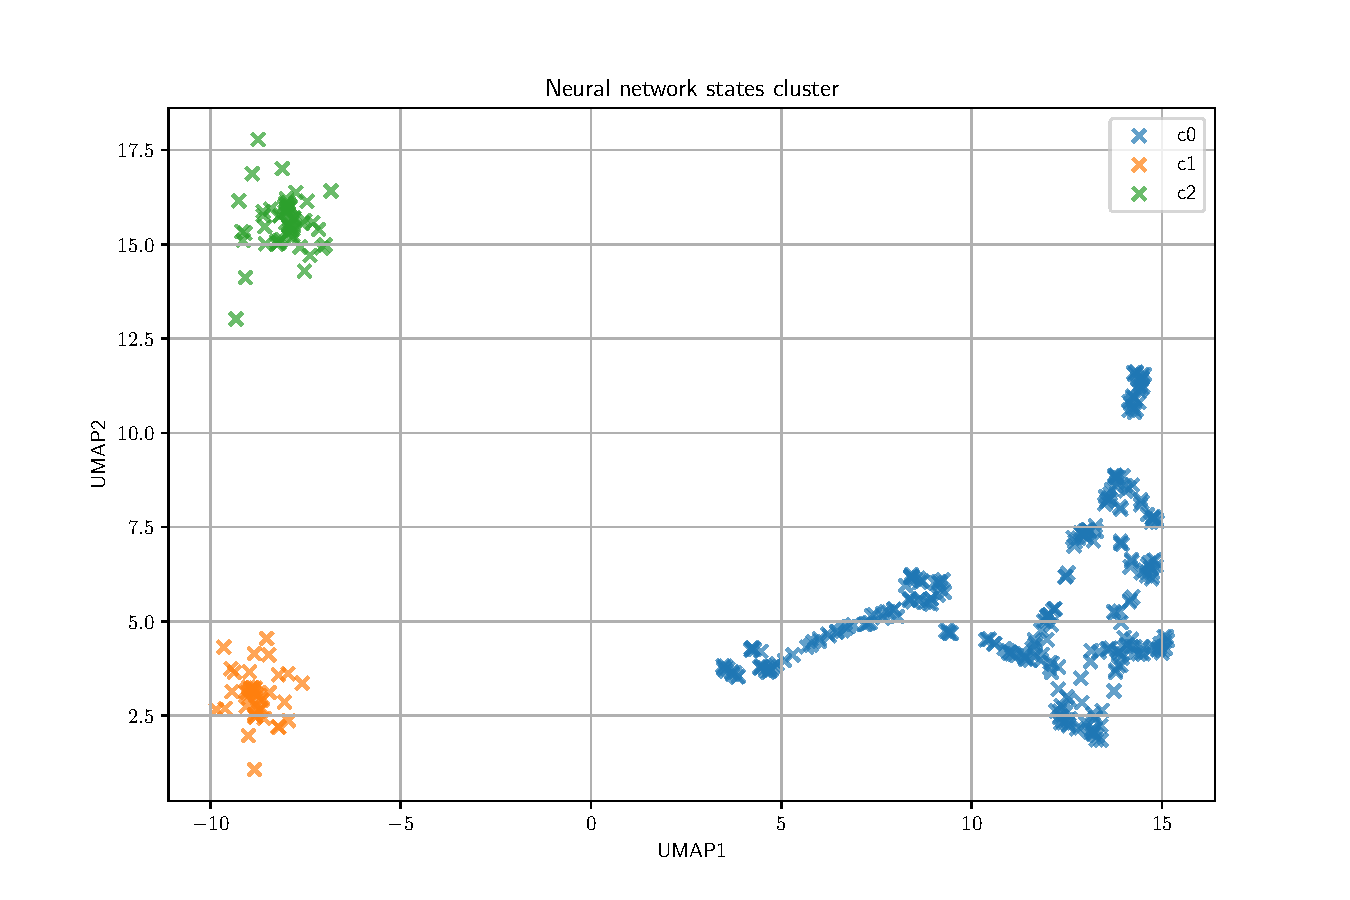
\includegraphics[width=1\linewidth]{umap.pdf}
  \caption{Распределение снимков весов, градиентов и гессианов в пространстве размерности 2}
  \label{fig:umap}
\end{figure}

На графике видно, что снимки из разных архитектур распределены в пространстве неравномерно, явно
распределяясь по кластерам. Это может указывать на то, что разные архитектуры имеют свои характерные паттерны
в весах, градиентах и гессианах, которые можно использовать для их классификации. Однако для более точной
интерпретации этих результатов требуется дальнейшее исследование.

\paragraph{Обобщённое практическое руководство.}
\begin{itemize}
  \item Пониженный ранг и симметричный спектр гессиана должны рассматриваться как предупреждающие сигналы:
    вероятны седловые точки, переизбыточность и ухудшение обобщения.
  \item Умеренная спектральная мощность и достаточно широкий спектр собственных значений указывают на
    «здоровое» многообразие направлений, которыми сеть учится, и, следовательно, на высокую потенцию к переносу знаний.
  \item Bias-параметры требуют регулярного мониторинга: процент их вклада в общий спектр гессиана служит
    метрикой отклонения от оптимальной геометрии.
  \item Анализ перекрёстной корреляции спектров весов, градиентов и гессиана позволяет своевременно
    обнаружить жёсткие направления и адаптировать план обучения (цикл learning rate, применить оптимизаторы
    второго порядка, добавить дифференциальную регуляризацию и~т.\,д.).
\end{itemize}

Таким образом, углублённый спектральный и ранговый анализ локальных гессианов — мощный диагностический
инструмент, позволяющий обнаруживать скрытые проблемы, формулировать рекомендации по корректировке
архитектуры и оптимизатора, а также количественно оценивать способность сети к обобщению.

\section{Обсуждение}
Проведённое исследование предлагает математически обоснованный инструмент для изучения внутренней динамики
нейронных сетей вместо проб и ошибок. Важным результатом является связь между геометрическими свойствами
параметрического пространства и функциональным поведением сети. Локальная кривизна, описываемая гессианом,
содержит информацию о режиме работы слоя и его вкладе в общую функциональность.

\begin{proposition}
  Исследование нейронной сети как композиции нелинейных операторов или хаотической динамической системы
  предоставляет наиболее информативные сведения о её внутренней структуре, механизмах обработки данных и
  математических ограничениях архитектуры.
\end{proposition}

Рассмотрение сети как динамической системы, эволюционирующей по многообразию высокой размерности с
нетривиальной геометрией, открывает новые горизонты для понимания и улучшения методов обучения.

В данном случае интересует именно развитие идеи с локальным гессианом в комбинации с римановой геометрией,
исследуя более детально геометрию локального пространства параметров. Это может помочь относительно быстро
находить места, где сеть может застревать.

\section{Заключение}
В данной работе предложен новый подход к анализу нейронных сетей через локальные свойства их параметрического
пространства, исследуемые с помощью матриц Гессе. Введённое понятие локального гессиана позволило:
\begin{itemize}
  \item Изучать геометрию функционального пространства отдельных слоёв;
  \item Выявлять закономерности распределения собственных значений в процессе обучения;
  \item Показать связь между спектром гессиана и насыщением активаций, формированием направлений и эволюцией
    представлений.
\end{itemize}

Стоит отметить масштаб проведённого эксперимента: было собрано около 1500 снимков состояний различных сетей
общей ёмкостью около 50 ГБ данных, что позволило выявить устойчивые закономерности.

Дальнейшие исследования могут включать:
\begin{itemize}
  \item Детальное изучение взаимосвязи спектральных свойств гессианов и функциональных характеристик слоёв;
  \item Анализ динамики спектра в процессе обучения и её связь с обобщающей способностью;
  \item Применение подхода к новым архитектурам — трансформерам, графовым сетям;
  \item Разработку методов визуализации и интерпретации геометрической структуры параметрического пространства.
\end{itemize}

\begin{thebibliography}{99}

  \bibitem{poole2016transient}
  B.~Poole, S.~Lahiri, M.~Raghu, J.~Sohl-Dickstein, and S.~Ganguli.
  \newblock Exponential expressivity in deep neural networks through transient chaos.
  \newblock In \emph{Advances in Neural Information Processing Systems}, pages 3360--3368, 2016.

  \bibitem{maheswaranathan2019universality}
  N.~Maheswaranathan, A.~H. Williams, M.~D. Golub, S.~Ganguli, and D.~Sussillo.
  \newblock Universality and individuality in neural dynamics across large populations of recurrent networks.
  \newblock In \emph{Advances in Neural Information Processing Systems}, 32, 2019.

  \bibitem{lee2019wide}
  J.~Lee, L.~Xiao, S.~S. Schoenholz, Y.~Bahri, R.~Novak, J.~Sohl-Dickstein, and J.~Pennington.
  \newblock Wide neural networks of any depth evolve as linear models under gradient descent.
  \newblock In \emph{Advances in Neural Information Processing Systems}, 32, 2019.

  \bibitem{arora2019finegrained}
  S.~Arora, S.~S. Du, W.~Hu, Z.~Li, and R.~Wang.
  \newblock Fine-grained analysis of optimization and generalization for overparameterized two-layer neural networks.
  \newblock In \emph{Proceedings of the 36th International Conference on Machine Learning}, pages 322--332, 2019.

  \bibitem{lecun2015deep}
  Y.~LeCun, Y.~Bengio, and G.~Hinton.
  \newblock Deep learning.
  \newblock \emph{Nature}, 521(7553):436--444, 2015.

  \bibitem{goodfellow2016deep}
  I.~Goodfellow, Y.~Bengio, and A.~Courville.
  \newblock \emph{Deep Learning}.
  \newblock MIT Press, 2016.

  \bibitem{sagun2017empirical}
  L.~Sagun, U.~Evci, V.~U. Güney, Y.~Dauphin, and L.~Bottou.
  \newblock Empirical analysis of the Hessian of over-parameterized neural networks.
  \newblock \emph{arXiv preprint arXiv:1706.04454}, 2017.

  \bibitem{ghorbani2019investigation}
  B.~Ghorbani, S.~Krishnan, and Y.~Xiao.
  \newblock An investigation into neural net optimization via Hessian eigenvalue density.
  \newblock In \emph{Proceedings of the 36th International Conference on Machine Learning}, pages 2232--2241, 2019.

  \bibitem{dangel2019modular}
  F.~Dangel, S.~Harmeling, and P.~Hennig,
  \newblock Modular block-diagonal curvature approximations for feedforward architectures.
  \newblock In \emph{arXiv preprint arXiv:1902.01813}, Feb. 2019.

  \bibitem{carlon2024}
  André G. Carlon, Luis Espath, Raúl Tempone.
  \newblock Approximating Hessian matrices using Bayesian inference: a new approach for quasi-Newton methods
  in stochastic optimization.
  \newblock In \emph{arXiv preprint arXiv:2208.00441v2}, 2024.

  \bibitem{hare2024}
  Warren Hare, Gabriel Jarry–Bolduc, Chayne Planiden.
  \newblock A matrix algebra approach to approximate Hessians.
  \newblock IMA Journal of Numerical Analysis, 44(4):2220–2250, 2024.

  \bibitem{martens2010}
  James Martens.
  \newblock Deep learning via Hessian-free optimization.
  \newblock In {\em Proc. 27th Int. Conf. Machine Learning (ICML)}, pages 735–742, 2010.

  \bibitem{nocedal1980}
  Jorge Nocedal.
  \newblock Updating Quasi-Newton Matrices with Limited Storage.
  \newblock Mathematics of Computation, 35(151):773–782, 1980.

  \bibitem{sagun2016}
  L.~Sagun, L.~Bottou, and Y.~LeCun,
  \newblock Eigenvalues of the Hessian in Deep Learning: Singularity and Beyond,
  \newblock In \emph{arXiv:1611.07476 [cs.LG]}, 2016.

  \bibitem{liaomahoney2021}
  Z.~Liao and M.~W.~Mahoney,
  \newblock Hessian Eigenspectra of More Realistic Nonlinear Models,
  \newblock In \emph{Advances in Neural Information Processing Systems}, vol.~34, 2021.

  \bibitem{shapiro1965}
  Shapiro, S.~S., \& Wilk, M.~B..
  \newblock An analysis of variance test for normality (complete samples).
  \newblock In \emph{Biometrika}, 52(3/4), 591–611, 1965.

\end{thebibliography}
\end{document}
